%************************************************
\chapter{Basic Concepts}\label{ch:introductionplanning}
%************************************************
General Introduction to Thesis

$\mathcal{C,W} = \mathbb{R}^2$

\section{Classic Path Planning Problem}\label{sec:basic}
Statespace,
Configurationspace,
Obstacles in Configurationspace,
Workspace,
Actions,
Paths,
Trajectories,

\section{Constraints on Motion}\label{sec:model}
The 

a) kinematic constraints
constraints on the velocities of a robot

Unconstrained or free:
The robot can move in any direction in the world. 

Holonomic:
A robot is called holonomic if all constraints can be expressed without using constraints on the velocity. 
A free moving robot with no constraints at all is holonomic.
A unicycle which can only move in one direction and is not allowed to change is orientation is also holonomic, since  it can be expressed without the use of derivates of state variables.
The formular is called a holonomic constraint.

Nonholonimc:
If state transitions can not be expressed without the use of velocities the system is called nonholonmic.
for example a robot with differential drive can roll forward and backward but not sideways. 
This no-slip constraint on the velocities of the vehicle is a noonholonimc constraint.
where velocities can not be removed by integration (reducing the dimension of the configuration space).
Therefore nonholonomic constraints are sometimes referred to as being non integrable.


The following example of a nonholonomic robot taken from Priciples of Robot Motion is a robot with differential drive illustrated in Figure \ref{fig_diff}.
The configuration of the robot is determined by its position and orientation q(x,y,phi).
The left and the rigth wheel can be actuated by a motor given the speeds $u_l$ and $u_r$.
This yields the following system.

This can not be integrated to eliminate x and y, hence the system is nonholonomic (see Planning algorithms).
  

Dynamic constraints:
Constraints on the acceleration of the vehicle.
Taking accelerations of vehicles into account the state also involves second derivatives of state variables.


\section{Representation of the Environment}\label{sec:representation}
Fixed Cell Decomposition
Exact Cell Decomposition
Approximate Cell Decomposition
Visibility Graph
Voronoi Regions

\section{Planning}\label{sec:global}
Global Planning:
Breadth-First Search (BFS)
Depth-First Search (DFS)
Dijkstra's and A* algorithm
An illustration is given in Figure~\ref{fig:fig_overview}
\begin{figure}[thpb]
	  \myfloatalign
      \footnotesize
      \centering
    \subfloat[Dijkstra algorithm]
    {  \label{fig:fig_djikstra}
        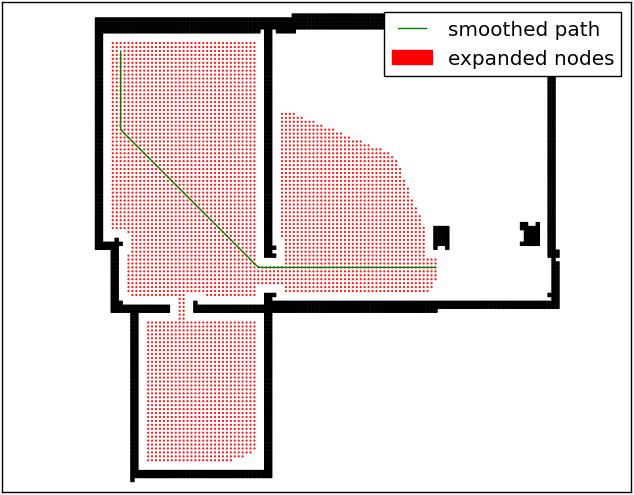
\includegraphics[width=0.75\textwidth]{figures/fig_djikstra.png}
        %\caption{Dijkstra}
    }
    
    \subfloat[A* algorithm]
    {  \label{fig:fig_astar}
       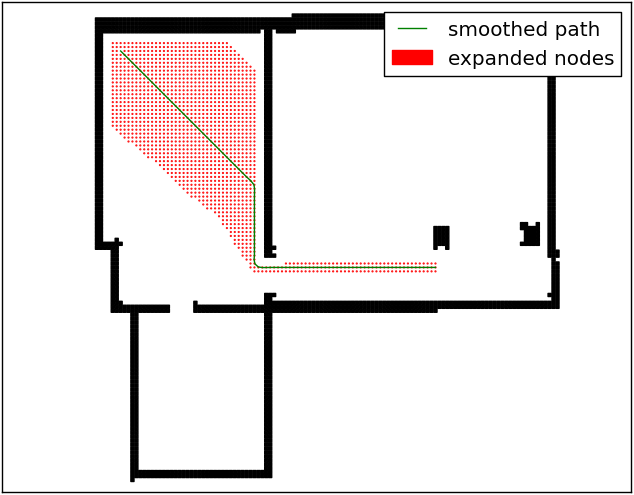
\includegraphics[width=0.75\textwidth]{figures/fig_astar.png}
       %\caption{A*}
    }
   \caption[Djikstra's and A* algorithm.]{The difference between Djikstra's and A* algorithm searching for a shortest path in a grid representation of a building. A* is more effective, as it visits by far less nodes in the search graph. }
\label{fig:fig_overview}
\end{figure}
Examples: 
Rapidly Exploring Randomized Trees (RRT)
Probabilistic Road Maps (PRM)
Potential Field
Meta-Heuristic approaches

Local Planning:
The next chapter investigates local planning methods.

%*****************************************
%*****************************************
%*****************************************
%*****************************************
%*****************************************




